\documentclass[11pt]{article}
\usepackage[fontsize = 12pt]{scrextend}
\usepackage{multicol}
\usepackage{multirow}
\usepackage{savesym}
\usepackage{hyperref}
\usepackage{amsmath}
\usepackage{algorithm}
\usepackage{algorithmic}
\usepackage{paralist}
\usepackage{float}
\usepackage[shortlabels]{enumitem}
\usepackage[bb=px]{mathalpha}
\usepackage[a4paper, margin=1in]{geometry}
\usepackage[dvipsnames]{xcolor}
\usepackage{tikz}
\newtheorem{theorem}{Theorem}
\usetikzlibrary{shapes,backgrounds}
\usetikzlibrary{positioning}
\title{SDS 383C - Statistical Modeling 1: Homework 1}
\author{Rahul Nandakumar \\ Graduate Student, ORIE Program (E-ID: rn9355)}
\date{September 11, 2022}
\begin{document}
\maketitle
\noindent 1. Prove Slutsky’s theorem (the version taught in class)\\ \\
\textbf{Solution:}
\begin{theorem}
  Let $\{x_{n}\}_{n = 1}^{\infty}$ and $\{z_{n}\}_{n = 1}^{\infty}$ be a sequence of random variables; $x$, $z$ be random variables; and $x_{0}, z_{0} \in \mathbb{R}$ be constants. Then,
  \begin{compactitem}
    \item $x_{n} \xrightarrow{P} x \Rightarrow x_{n} \xrightarrow{D} x,$
    \item $x_{n} \xrightarrow{D} x_{0} \Rightarrow x_{n} \xrightarrow{P} x_{0},$
    \item $x_{n} \xrightarrow{D} x$ and $z_{n} \xrightarrow{P} z_{0} \Rightarrow $\\
    $x_{n} + z_{n} \xrightarrow{D} x + z_{0}$, $x_{n}z_{n} \xrightarrow{D} xz_{0}$, $x_{n}/z_{n} \xrightarrow{D} x/z_{0} (z_{0} \neq 0)$
  \end{compactitem}
\end{theorem}
\textbf{Proof:}
From the statements given to us, we can write the following.
\begin{equation}
  \nonumber
  \begin{aligned}
    F_{x_{n} + z_{n}}(t) = P[x_{n} + z_{n} \leq t, z_{n} \geq z_{0} - \epsilon] + P[x_{n} + z_{n} \leq t, z_{n} < z_{0} - \epsilon]
  \end{aligned}
\end{equation}
Let t be a point of continuity of $F_{x + z_{0}}$. Because a distribution function has atmsot countable many points of discontinuity, we can choose $\epsilon$ positive for any $t$ such that $t +  \epsilon$ are both points of continuity of $F_{x + z_{0}}$. We now get
\begin{equation}
  \nonumber
  F_{x_{n} + z_{n}}(t) \leq P[x_{n}  \leq t - z_{0} + \epsilon] + P[ \lvert z_{n} - z_{0} \rvert > \epsilon]
\end{equation}
Furthermore, we have
\begin{equation}
  \nonumber
  P[x_{n}  \leq t - z_{0} + \epsilon] = F_{x_{n} + z_{0}}(t + \epsilon)
\end{equation}
Now because $F_{x_{n} + z_{0}}(t) = P[x_{n}  \leq t - z_{0}] = F_{x_{n}}(t - z_{0}) $, we must have $x_{n} + z_{0} \xrightarrow{D} x + z_{0}$. This leads to the following relationship,
\begin{equation}
  \nonumber
  \underset{n}{\text{lim sup }}F_{x_{n} + z_{n}}(t) \geq \underset{n}{\text{lim}}F_{x_{n} + z_{0}}(t + \epsilon) + \underset{n}{\text{lim}}P[\lvert z_{n} - z_{0} \rvert \geq \epsilon] = F_{(x + z_{0})}(t + \epsilon)\\
\end{equation}Similarly,
\begin{equation}
  \nonumber
  1 - \underset{n}{\text{lim sup }}F_{x_{n} + z_{n}}(t) = P[x_{n} + z_{n} > t] \leq P[x_{n} > t - z_{0} -\epsilon] + P[\lvert z_{n} - z_{0} \rvert > \epsilon]
\end{equation}
and hence, we get
\begin{equation}
  \nonumber
  \underset{n}{\text{lim inf }}F_{x_{n} + z_{n}}(t) \geq \underset{n}{\text{lim}}F_{x_{n} + z_{0}}(t - \epsilon) = F_{x + z_{0}}(t - \epsilon)
\end{equation}
Therefore, we can say that
\begin{equation}
  \nonumber
  F_{x + z_{0}}(t - \epsilon) \leq \underset{n}{\text{lim inf }}F_{x_{n} + z_{n}}(t) \leq \underset{n}{\text{lim sup }}F_{x_{n} + z_{n}}(t) \leq F_{(x + z_{0})}(t + \epsilon)
\end{equation}
From the above equation, since $\epsilon$ can reach 0 and $F_{x + z_{0}}$ is continuous at t, we can conclude that $x_{n} + z_{n} \xrightarrow{D} x + z_{0}$. A simplified version of these statements is that if $x_{n}$ converges in distribution to $x$ and $z_{n}$ converges in probability to $z_{0}$, then their joint vector $(x_{n}, z_{n})$ converges in distribution to $(x, z_{0})$. By applying continuous mapping further, where $g(x, y) = x + y$, we get
\begin{equation}
  \nonumber
  x_{n} + z_{n} \xrightarrow{D} x + z_{0}
\end{equation}
Furthermore, if $g(x, y) = xy$, we get
\begin{equation}
  \nonumber
  x_{n}z_{n} \xrightarrow{D} xz_{0}
\end{equation}
And if $g(x, y) = x/y$,
\begin{equation}
  \nonumber
  x_{n}/z_{n} \xrightarrow{D} x/z_{0}
\end{equation}
(Source: Mathematical Statistics: Basic Ideas and Selected Topics Volume 1 by Bickel and Doksum)\\ \\
\noindent 2. For $y \sim \text{Poisson}(\lambda)$, show that $\mathbb{E}(y) = var(y) = \lambda$. Method of moments suggests $\bar y_{n}$ the sample mean, as well as $s_{n}^{2}$, the sample variance, could both be reasonable estimators of $\lambda$. Which one would you prefer? Why?\\ \\
\textbf{Solution:} We are given, $y \sim \text{Poisson}(\lambda)$. The PMF of this distribution is given by $P(Y = y) = \frac{e^{-\lambda}\lambda^{y}}{y!}$ Now, let us find the Moment Generating Function of the Poisson Distribution.
\begin{equation}
  \begin{aligned}
    M_{y}(t) & = \mathbb{E}(e^{ty})\\
    & = e^{t.0}(P(y = 0)) + e^{t.1}(P(y = 1)) + \dots \\
    & = 1.e^{\lambda} + e^{t}.e^{-\lambda}.\frac{\lambda}{1!} + e^{2t}.e^{-\lambda}.\frac{\lambda^{2}}{2!} + \dots\\
    & = e^{-\lambda}.e^{k}, \text{ where } k = e^{t}\lambda \\
    & = e^{-\lambda} e^{e{t}\lambda}\\
    & = e^{\lambda(e^{t} - 1)}
  \end{aligned}
\end{equation}
Using the result in (1), we can calculate the first and second order moments as follows. The first order moment can be calulated as
\begin{equation}
  \nonumber
  \begin{aligned}
    M^{1}(t) & = \frac{dM(t)}{dt}\\
    & = \frac{d}{dt}\bigg[e^{\lambda(e^{t} - 1)}\bigg]\\
    & = e^{\lambda(e^{t} - 1)} \times (\lambda e^{t})
  \end{aligned}
\end{equation}
The second order moment can be calculated as follows.
\begin{equation}
  \nonumber
  \begin{aligned}
    M^{2}(t) & = \frac{d^{2}M(t)}{dt^{2}}\\
    & = \frac{d}{dt}\bigg[\frac{d}{dt}\bigg[e^{\lambda(e^{t} - 1)}\bigg]\bigg]\\
    & = e^{\lambda(e^{t} - 1)}(\lambda e^{t}) + (\lambda e^{t})\bigg[e^{\lambda(e^{t} - 1)}.\lambda e^{t}\bigg]\\
    & = (e^{\lambda(e^{t} -1)}\lambda e^{t})\bigg[1 + \lambda e^{t}\bigg]
  \end{aligned}
\end{equation}
Now, we can calculate the first order and second order moment values at $t = 0$ to get $\mathbb{E}(y)$ and $\mathbb{E}(y^{2})$ respectively. Therefore,
\begin{equation}
  \begin{aligned}
    \mathbb{E}(y) & = M^{1}(t) \rvert_{t = 0}\\
    & = e^{\lambda(e^{t} - 1)} \times (\lambda e^{t}) \bigg\rvert_{t = 0}\\
    & = e^{\lambda(e^{0} - 1)} \times (\lambda e^{0})\\
    & = \lambda
  \end{aligned}
\end{equation}
\begin{equation}
  \begin{aligned}
    \mathbb{E}(y^{2}) & = M^{2}(t) \rvert_{t = 0}\\
    & = (e^{\lambda(e^{t} -1)}\lambda e^{t})\bigg[1 + \lambda e^{t}\bigg] \rvert_{t = 0}\\
    & = (e^{\lambda(e^{0} -1)}\lambda e^{0})\bigg[1 + \lambda e^{0}\bigg]\\
    & = \lambda(1 + \lambda) = \lambda + \lambda^{2}
  \end{aligned}
\end{equation}
Now, we know that $var(y) = \mathbb{E}(y^{2}) - (\mathbb{E}(y))^{2}$. Therefore, from (2) and (3), we can write
\begin{equation}
  var(y) = \mathbb{E}(y^{2}) - (\mathbb{E}(y))^{2} = \lambda^{2} + \lambda - \lambda^{2} = \lambda
\end{equation}
From (4), we have shown that for a poission distribution with shape parameter $\lambda$, $\mathbb{E}(y) = var(y) = \lambda$. We can see that by using the method of moments, both the sample mean $(\bar y_{n})$ and sample variance $(s_{n}^{2})$ are reasonable estimators of $\lambda$. In this case, we can say that the $\mathbb{E}(y)$ is a better estimator of $\lambda$ because we know that for any distribution, $\mathbb{E}(y)$ is an unbiased estimate of population mean $\mu$ (or in this case $\lambda$). Also, we find that for a Poission Distribution, the sample mean is a sufficient statistic and is therefore a much better estimator for $\lambda$. It is also much easier to compute $\mathbb{E}(y)$.\\ \\

\noindent 3. For $(x_{1}, y_{1}), (x_{2}, y_{2}), \dots, (x_{n}, y_{n}) \overset{iid} \sim f_{x,y}$ with finite second order moments. Show that the sample correlation coefficient $r_{n}$ converges in probability to the population correlation coefficient $\rho$. \\ \\
\textbf{Solution:} For any $(x_{1}, y_{1}), (x_{2}, y_{2}), \dots, (x_{n}, y_{n}) \overset{iid} \sim f_{x,y}$ with finite second order moments, the sample correlation coefficient is given by
\begin{equation}
  \nonumber
  r_{n} = \frac{\sum_{i = 1}^{n}(y_{i} - \bar{y})(x_{i} - \bar{x})}{\{\sum_{i = 1}^{n}(y_{i} - \bar{y})^{2}\sum_{i = 1}^{n}(x_{i} - \bar{x})^{2}\}^{1/2}}
\end{equation}
Now, we divide and multiply $r_{n}$ with $n$. We get,
\begin{equation}
  \nonumber
    r_{n} = \frac{\frac{\sum_{i = 1}^{n}(y_{i} - \bar{y})(x_{i} - \bar{x})}{n}}{\{\frac{\sum_{i = 1}^{n}(y_{i} - \bar{y})^{2}}{n}\frac{\sum_{i = 1}^{n}(x_{i} - \bar{x})^{2}}{n}\}^{1/2}}
\end{equation}
For the numerator, we have
\begin{equation}
  \nonumber
  N = \frac{\sum_{i = 1}^{n}(y_{i} - \bar{y})(x_{i} - \bar{x})}{n}
\end{equation}
Now, as $n \xrightarrow{} \infty$, $N \xrightarrow{P} \sigma_{xy}$. Similarly, we have
\begin{equation}
  \nonumber
  \begin{aligned}
    D & = \{\frac{\sum_{i = 1}^{n}(y_{i} - \bar{y})^{2}}{n}\frac{\sum_{i = 1}^{n}(x_{i} - \bar{x})^{2}}{n}\}^{1/2}\\
    & = D_{1} \times D_{2}
  \end{aligned}
\end{equation}
Where $D_{1} = \{\frac{\sum_{i = 1}^{n}(y_{i} - \bar{y})^{2}}{n}\}^{1/2}$ and $D_{2} = \{\frac{\sum_{i = 1}^{n}(x_{i} - \bar{x})^{2}}{n}\}^{1/2}$ As $n \xrightarrow{} \infty$, we have $D_{1} \xrightarrow{P} \sigma_{y}$ and $D_{2} \xrightarrow{P} \sigma_{x}$. Therefore, we can say that $D \xrightarrow{P} \sigma_{x}\sigma_{y}$.\\ \\
We make use of the property of continuous mapping theorem, which states that if $x_{n} \xrightarrow{P} x$, then $g(x_{n}) \xrightarrow{P} g(x)$ for $\{x_{n}\}_{n=1}^{\infty}$
a sequence of random variables and $g$ be any function with $D_{g}$ points of discontinuity.\\ \\
Now, we have
\begin{equation}
  \nonumber
  \begin{aligned}
    r_{n} & = \frac{N}{D}\\
    & \xrightarrow{P} \frac{\sigma_{xy}}{\sigma_{x}\sigma_{y}}\\
    & = \rho
  \end{aligned}
\end{equation}
Therefore, we have shown that $r_{n} \xrightarrow{P} \rho$ as $n \xrightarrow{} \infty$
\\ \\
\noindent 4. Notations having their usual significance, for $y_{1}, \dots, y_{n} \overset{iid}\sim Ga(\alpha, \beta)$, a method of moment estimator of $\alpha$ is $\hat{\alpha} = \bar{y_{n}}^{2}/s_{n}^{2}$. Using the multivariate delta method, show that $SE(\hat{\alpha}) = \sqrt{2\alpha(\alpha+1)/n}$ for large values of n.\\ \\
\textbf{Solution:} Method of moments gives us an estimate of $\alpha$, which is $\hat{\alpha} = \bar{y_{n}}^{2}/s_{n}^{2}$. We also know that $\hat{\beta} = \bar{y_{n}}/s_{n}^{2}$ Let $t_{1n} = \bar{y_{n}}$ and $t_{n2} = s_{n}^{2}$. We have proved in the class the following results.
\begin{equation}
  \nonumber
  \begin{aligned}
    var(\bar{y_{n}}) & = \frac{\alpha}{\beta^{2}n}\\
    var(s_{n}^{2}) & = \frac{6\alpha}{\beta^{4}n} + \frac{2\alpha^{2}}{\beta^{4}n}\\
    cov(\bar{y_{n}}, s_{n}^{2}) & = \frac{2\alpha}{\beta^{3}n}
  \end{aligned}
\end{equation}
Using the conclusion from the multivariate delta method, which is stated as follows
\begin{equation}
  \nonumber
  \sqrt{n}\{h(\mathbf{t_{n}}) - h(\mathbf{\theta})\} \xrightarrow{D} \text{Normal}\{\mathbf{0}, h^{'}(\mathbf{\theta})^{T}\mathbf{\text{$ \sum$}}h^{'}(\mathbf{\theta})\}
\end{equation}
Here, we have
\begin{equation}
  \nonumber
  \begin{aligned}
    \hat{\alpha_{n}} & = \bar{y_{n}}^{2}/s_{n}^{2}\\
    h(t_{1n}, t_{2n}) & = \frac{t_{1n}^{2}}{t_{2n}}
  \end{aligned}
\end{equation}
Now, we can calculate $h^{'}(\theta)$ by taking the partial derivative of $h(t_{1n}, t_{2n})$ wrt. $t_{1n}$ and $t_{2n}$. This yields.
\begin{equation}
  \nonumber
  \begin{aligned}
    \frac{\partial h}{\partial t_{1n}} &= \frac{2t_{1n}}{t_{2n}}\\
    \frac{\partial h}{\partial t_{1n}} \bigg\rvert_{\theta}  & = 2\beta; \text{ Since from the result of } \hat{\beta_{n}}
  \end{aligned}
\end{equation}
\begin{equation}
  \nonumber
  \begin{aligned}
    \frac{\partial h}{\partial t_{2n}} &= \frac{-t_{1n}^{2}}{t_{2n}^{2}}\\
    \frac{\partial h}{\partial t_{2n}} \bigg\rvert_{\theta}  & = -\beta^{2}; \text{ Since from the result of } \hat{\beta_{n}}
  \end{aligned}
\end{equation}
Therefore $h^{'}(\theta) = (2\beta, -\beta^{2})$. Using this result, we can calculate $var(\bar{y}_{n}^{2}/s_{n}^{2})$
\begin{equation}
  \nonumber
  \begin{aligned}
      var(\bar{y}_{n}/s_{n}^{2}) & =  h^{'}(\mathbf{\theta})^{T}\mathbf{\text{$ \sum$}}h^{'}(\mathbf{\theta})\\
      & = (2\beta, -\beta^{2}) \begin{pmatrix}
        \frac{\alpha}{\beta^{2}n} & \frac{2\alpha}{\beta^{3}n}\\
        \frac{2\alpha}{\beta^{3}n} & \frac{6\alpha}{\beta^{4}n} + \frac{2\alpha^{2}}{\beta^{4}n}
    \end{pmatrix}
    \begin{pmatrix}
      2\beta\\
      -\beta^{2}
    \end{pmatrix}\\
    & = \begin{pmatrix}
      0 & \frac{4\alpha}{\beta^{2}n} - \frac{6\alpha}{\beta^{2}n} - \frac{2\alpha^{2}}{\beta^{2}n}
  \end{pmatrix}\begin{pmatrix}
    2\beta\\
    -\beta^{2}
\end{pmatrix}\\
& = \frac{2\alpha(\alpha + 1)}{n}
  \end{aligned}
\end{equation}
Since we are asked to find $SE(\hat{\alpha}_{n})$, we get
\begin{equation}
  \nonumber
  \begin{aligned}
    SE(\hat{\alpha}_{n}) & = SE(\bar{y}_{n}/s_{n}^{2})\\
    & = \sqrt{var(\bar{y}_{n}/s_{n}^{2})}\\
    & = \sqrt{\frac{2\alpha(\alpha + 1)}{n}}
  \end{aligned}
\end{equation}
\noindent 5. Now fix the values of $\alpha$ and $\beta$. For your chosen values of $\alpha$ and $\beta$, draw a random sample of size of $n=50$ from a $Ga(\alpha, \beta)$ distribution. Using method of moments and assuming $\alpha$ and $\beta$ to now be unknown, estimate $\alpha$, $\beta$. Plot the histogram of the samples, superimposed with the true density and the estimated density. \\
Repeat the above procudure B = 50, 500 and 1000 times. Plot a histogram of $\sqrt{n}\frac{(\hat{\alpha}_{n} - \alpha)}{\sqrt{2 \hat{\alpha}_{n}(\hat{\alpha}_{n} + 1)}}$ for each of the above values of B. In each case, superimpose a Normal (0,1) distribution over the histogram. For your final output, provide a very brief description of what you did, the plots, the codes and your general comments, if any.\\ \\
\textbf{Solution:} Using method of moments, we arrive at the estimators of $\hat{\alpha}_{n}$ and $\hat{\beta}_{n}$ as follows.
\begin{equation}
  \nonumber
  \begin{aligned}
    \hat{\alpha}_{n} & = \frac{{\bar{y}_{n}}^{2}}{{s_{n}}^{2}}\\
    \hat{\beta}_{n} & = \frac{{\bar{y}_{n}}}{{s_{n}}^{2}}
  \end{aligned}
\end{equation}
Now, we generate a random sample from a Gamma distribution with shape $\alpha$ and rate $\beta$ with population size $n = 100000$. We assume $\alpha = 4$ and $\beta = 0.6$. We first generate a sample of 50 numbers from this population. We have 3 functions in our code, namely \emph{estimators}, \emph{plot}, \emph{mvd\_plotting}. The function \emph{estimator} takes in the value of $\alpha$ and $\beta$, along with the sample size and generates a Gamma functions. Further, it estimates the value of $\alpha$ as $\hat{\alpha}$ and $\beta$ as $\hat{\beta}$ and returns these values. The \emph{plot} function takes in these values, and generates the estimated density, actual density and a histogram of the samples. For large values of n, we find that the method of moments way of estimating the parameters $\alpha$ and $\beta$ is pretty accurate. This can be understood from the plot below.
\begin{figure}[H]
  \centering
  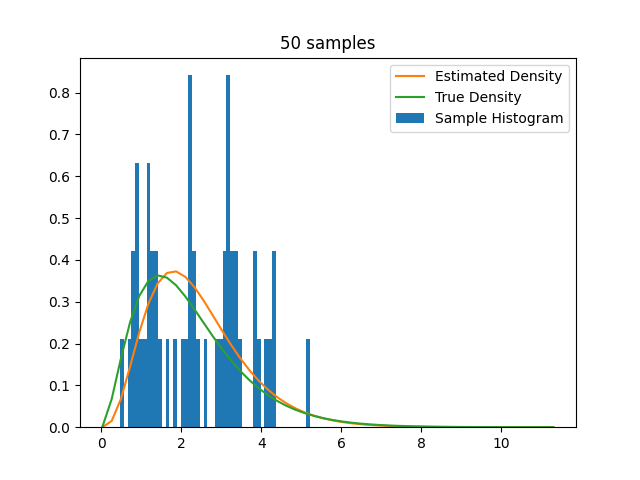
\includegraphics[width = 0.8\textwidth]{5.1.png}
  \caption{Estimated Density, True Density and sample histogram for a sample size of 50.}
\end{figure}
\noindent Now, we repeat the procudure of sampling from the gamma distribution and estimating $\alpha$ for $B = 50, 100, 500$ times. We calculate the value of $\sqrt{n}\frac{(\hat{\alpha}_{n} - \alpha)}{\sqrt{2 \hat{\alpha}_{n}(\hat{\alpha}_{n} + 1)}}$ and plot a histogram of it superimposed with a Normal(0,1) distribution.
\begin{figure}[H]
  \centering
  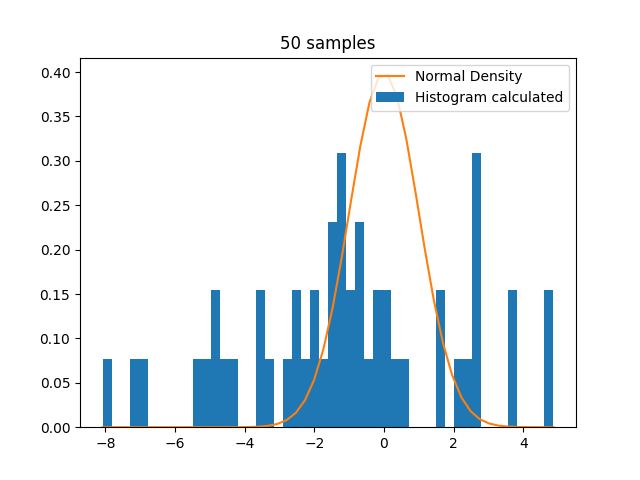
\includegraphics[width = 0.5\textwidth]{5.2.png}
  \caption{$B = 50$, plot of Normal(0,1) vs Histogram of calculated values.}
\end{figure}
\begin{figure}[H]
  \centering
  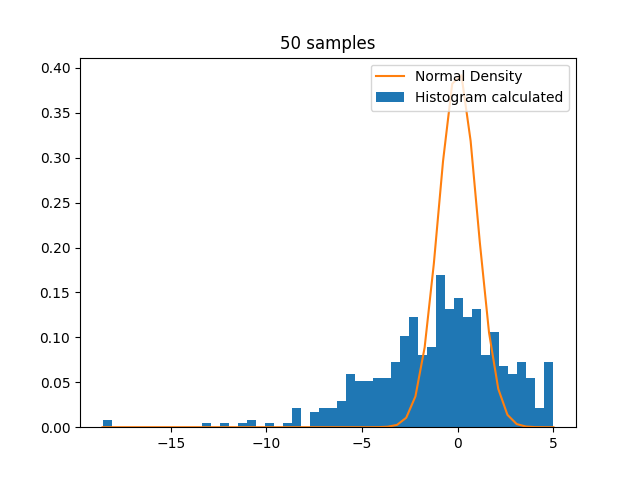
\includegraphics[width = 0.5\textwidth]{5.3.png}
  \caption{$B = 500$, plot of Normal(0,1) vs Histogram of calculated values.}
\end{figure}
\begin{figure}[H]
  \centering
  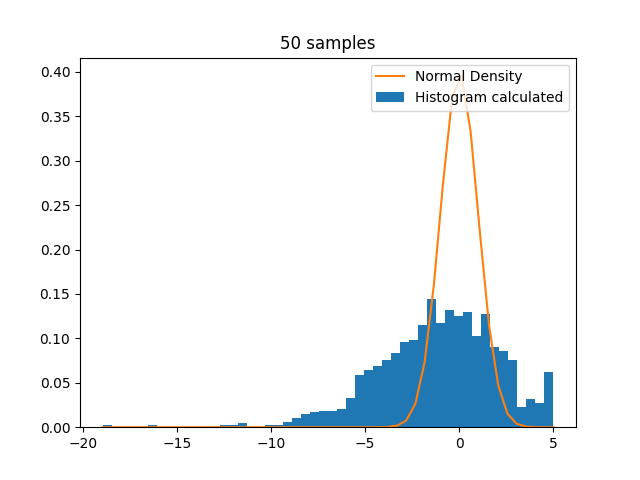
\includegraphics[width = 0.5\textwidth]{5.4.png}
  \caption{$B = 1000$, plot of Normal(0,1) vs Histogram of calculated values.}
\end{figure}
\noindent We get 3 results as illustrated above. We can thus conclude that for large values of sample numbers, the distribution of $\sqrt{n}\frac{(\hat{\alpha}_{n} - \alpha)}{\sqrt{2 \hat{\alpha}_{n}(\hat{\alpha}_{n} + 1)}}$ will converge to Normal(0, 1).\\ \\
\noindent 6. For a Normal$(\mu, \sigma^{2})$ distribution, show that the MGF is $M(t) = exp(\mu t + \sigma^{2}t^{2}/2)$\\ \\
\textbf{Solution:} We know that the PMF of a Normal distribution with mean $\mu$ and standard deviation $\sigma$ is given by
\begin{equation}
  \nonumber
  \begin{aligned}
    P(Y = y) & = \frac{1}{\sqrt{2\pi}{\sigma}}e^{\frac{-1}{2\sigma^{2}}(y  - \mu)^{2}}\\
  \end{aligned}
\end{equation}
The moment generating function is given as $M(t) = \mathbb{E}(e^{ty})$. Therefore, we can write it as follows.
\begin{equation}
  \nonumber
  \begin{aligned}
    M(t) & = \mathbb{E}(e^{ty})\\
    & = \int_{-\infty}^{\infty}e^{ty}f(y)dy\\
    & = \int_{-\infty}^{\infty}e^{ty}\frac{1}{\sqrt{2\pi}{\sigma}}e^{\frac{-1}{2\sigma^{2}}(y  - \mu)^{2}}dy\\
    & = \frac{\sqrt{2}\sigma}{\sqrt{2\pi}\sigma}\int_{-\infty}^{\infty}e^{t(\sqrt{2}z\sigma+\mu)-z^{2}}dz; \text{ Substituting } \frac{y - \mu}{\sqrt{2}\sigma} = z\\
    & = \frac{e^{\mu t}}{\sqrt{\pi}}\int_{-\infty}^{\infty}e^{-(z - \frac{\sqrt{2}}{2}\sigma t)^{2} + \frac{1}{2}\sigma^{2}t^{2}} dz\\
    & = \frac{e^{\mu t + \frac{1}{2}\sigma^{2}t^{2}}}{\sqrt{\pi}} \int_{-\infty}^{\infty}e^{-x^{2}}dx; \text{ Substituting } z - \frac{\sqrt{2}}{2}\sigma t = x\\
    & =  \frac{e^{(\mu t + \frac{1}{2}\sigma^{2}t^{2})}\sqrt{\pi}}{\sqrt{\pi}}; \text{ Since }\int_{-\infty}^{\infty}e^{-x^{2}}dx = \sqrt{\pi}\\
    & = e^{(\mu t + \frac{1}{2}\sigma^{2}t^{2})}
  \end{aligned}
\end{equation}
Therefore we have shown that for a Normal$(\mu, \sigma^{2})$ distribution, the MGF is $M(t) = exp(\mu t + \sigma^{2}t^{2}/2)$\\ \\
\noindent 7. Show that a binomial random variable $R$ with denominator $m$ and probability $\pi$ has a cumulant generating function $K(t) = m \text{log}(1 - \pi + \pi e^{t})$. Find lim $k(t)$ as $m \xrightarrow{} \infty, \pi \xrightarrow{} 0$ in a way so that $m\pi \xrightarrow{} \lambda > 0$. Show that
\begin{equation}
  \nonumber
  Pr(R = r) = \frac{\lambda^{r}}{r!}e^{-\lambda}
\end{equation}
and hence establish $R \xrightarrow{D} \text{Poisson}(\lambda)$. Using your favorite programming language, provide a numerical illustration of the result.\\ \\
\textbf{Solution:} We are given that $R$ is a binomial random variable with denominator $m$ and probability $\pi$. Therefore, we can write the probability mass function as follows.
\begin{equation}
  \nonumber
  Pr(R = r) = ^{m}C_{r} \pi^{r}(1-\pi)^{m-r}
\end{equation}
Now, we calculate the moment generating function of this probability distribution. We have,
\begin{equation}
  \nonumber
  \begin{aligned}
    M(t) & = \mathbb{E}(e^{tr})\\
    & = \sum_{r = 0}^{m} \frac{m!}{(m-r!)r!} \pi^{r}(1-\pi)^{m-r}.e^{tr}\\
    & = \sum_{r = 0}^{m} \frac{m!}{(m-r!)r!} (\pi e^{t})^{r}(1 - \pi)^{m-r}\\
    & = (1-\pi)^{m} + \frac{m}{1!}(1-\pi)^{m-1}(\pi e^{t}) + \frac{m(m-1)}{2!}(1-\pi)^{m-2}(\pi e^{t})^{2} + \dots + (\pi e^{t})^{m}\\
    & = \big[\pi e^{t} + (1 - \pi)\big]^{m}; \text{ By using the property of binomial expansion}\\
  \end{aligned}
\end{equation}
Now, we have the moment generating function of a binomial distribution. Using this, we can find the cumulant generating function as follows.
\begin{equation}
  \nonumber
  \begin{aligned}
    K(t) & = \text{log } M(t) \\
    & = \text{log} \big[\pi e^{t} + (1 - \pi)\big]^{m}\\
    & = m \text{log} \big[\pi e^{t} + (1 - \pi)\big]
  \end{aligned}
\end{equation}
Thus, we have shown that the cumulant generating function for a binomial distribution is given by $m \text{log} \big[\pi e^{t} + (1 - \pi)\big]$. Now, we need to find the limit as asked.
\begin{equation}
  \nonumber
  \begin{aligned}
    \underset{{m \xrightarrow{} \infty, \pi \xrightarrow{} 0}}{\text{lim}} K(t) & = \underset{{m \xrightarrow{} \infty, \pi \xrightarrow{} 0}}{\text{lim}} m \text{log} \big[\pi e^{t} + (1 - \pi)\big]
  \end{aligned}
\end{equation}
Let us assume $m \pi \xrightarrow{} \lambda$. Therefore, $ \pi = \frac{\lambda}{m}$. Therefore, we can write
\begin{equation}
  \nonumber
  \begin{aligned}
    \underset{{m \xrightarrow{} \infty, \pi \xrightarrow{} 0}}{\text{lim}} K(t) & = \underset{{m \xrightarrow{} \infty, \pi \xrightarrow{} 0}}{\text{lim}} m \text{log} \bigg[\frac{\lambda}{m} e^{t} + (1 - \frac{\lambda}{m})\bigg]\\
    & = \underset{{m \xrightarrow{} \infty}}{\text{lim}}\text{log}\bigg(1 + \frac{\lambda(e^{t} - 1)}{m}\bigg)^{m}\\
    & = \text{log}(e^{\lambda(e^{t} - 1)}); \text{ Applying } \underset{{m \xrightarrow{} \infty}}{lim} (1 + \frac{x}{n})^{n} = e^{x}\\
    & = \lambda(e^{t} - 1)
  \end{aligned}
\end{equation}
Following this, we now try to establish that $R \xrightarrow{D} \text{Poisson}(\lambda)$
\begin{equation}
  \nonumber
  \begin{aligned}
    P(R = r) & = \frac{m!}{(m-r)!r!} \bigg(\frac{\lambda}{m}\bigg)^{r} \bigg(1 - \frac{\lambda}{m}\bigg)^{m-r}\\
    \underset{{m \xrightarrow{} \infty}}{\text{lim}} P(R = r) & = \underset{{m \xrightarrow{} \infty}}{\text{lim}} \frac{m!}{(m-r)!r!} \bigg(\frac{\lambda}{m}\bigg)^{r} \bigg(1 - \frac{\lambda}{m}\bigg)^{m-r}\\
    & = \frac{\lambda^{r}}{r!}\underset{{m \xrightarrow{} \infty}}{\text{lim}}\frac{m!}{(m-r)!r!} \bigg(1 - \frac{\lambda}{m}\bigg)^{m} \bigg(1 - \frac{\lambda}{m}\bigg)^{-r} \bigg(\frac{1}{m}\bigg)^{r}
  \end{aligned}
\end{equation}
We look at each part of the limit individually. First, we have
\begin{equation}
  \nonumber
  \begin{aligned}
    \underset{{m \xrightarrow{} \infty}}{\text{lim}} \frac{m!}{(m-r)!r!}\bigg(\frac{1}{m^r}\bigg) & = \underset{{m \xrightarrow{} \infty}}{\text{lim}} \frac{m(m-1)(m-2)\dots(3)(2)(1)}{(m-r)(m-r-1)(m-r-2) \dots (3)(2)(1)} \bigg(\frac{1}{m^r}\bigg)\\
    & = \underset{{m \xrightarrow{} \infty}}{\text{lim}} \frac{m(m-1)(m-2) \dots (m-r+1)}{m^r}; \text{ Cancelling out denominator terms}\\
    & = \underset{{m \xrightarrow{} \infty}}{\text{lim}} \bigg(\frac{m}{m}\bigg)\bigg(\frac{m-1}{m}\bigg)\dots\bigg(\frac{m-r+1}{m}\bigg)\\
    & = 1
  \end{aligned}
\end{equation}
Now for the second part, we have
\begin{equation}
  \nonumber
  \begin{aligned}
    \underset{{m \xrightarrow{} \infty}}{\text{lim}} \bigg(1 - \frac{\lambda}{m}\bigg)^{m} = e^{\lambda}; \text{ Here, } x = -\lambda \text{ and } \underset{{n \xrightarrow{} \infty}}{\text{lim}} \bigg(1 + \frac{x}{n}\bigg) = e^{x}
  \end{aligned}
\end{equation}
Also, we have
\begin{equation}
  \nonumber
  \begin{aligned}
    \underset{{m \xrightarrow{} \infty}}{\text{lim}} \bigg(1 - \frac{\lambda}{m}\bigg)^{-r} = 1; \text{ as } \frac{\lambda}{m} \xrightarrow{} 0
  \end{aligned}
\end{equation}
Therefore, we obtain the result,
\begin{equation}
  \nonumber
  \begin{aligned}
    \underset{{m \xrightarrow{} \infty}}{\text{lim}} \frac{m!}{(m-r)!r!}\bigg(\frac{\lambda}{m}\bigg)^{r} \bigg(1 - \frac{\lambda}{m}\bigg)^{m-r} & = \frac{e^{-\lambda}\lambda^{r}}{r!}\\
    \underset{{m \xrightarrow{} \infty}}{\text{lim}}\frac{m!}{(m-r!)r!} \pi^{r}(1-\pi)^{m-r} & = \frac{e^{-\lambda}\lambda^{r}}{r!}
  \end{aligned}
\end{equation}
And we can say that
\begin{equation}
  \nonumber
  Pr(R = r) = \frac{\lambda^{r}}{r!}e^{-\lambda}
\end{equation}
Graphically, we arrive at the following result. For $m = 10000$ and $\pi = 0.4$, we get the following distribution
\begin{center}
  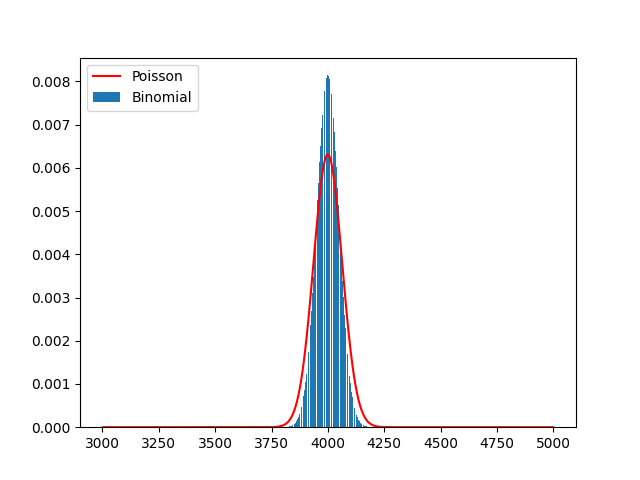
\includegraphics[width=\textwidth]{binompoisson.png}
\end{center}
We find that as the sample size $m$ is large, the Binomial distribution (in blue) converges to the Poisson Distribution (in red). The mean of the Poisson Distribution is $m \times \pi = 10000 \times 0.4 = 4000$. This is also in agreement with our mathematical derivation. \\ \\
\noindent 8. If $Z \sim \text{Normal}(0,1)$, derive the density of $Y = Z^{2}$. Although $Y$ is determined by $Z$, show that they are uncorrelated.\\ \\
\textbf{Solution:} It is given that $Z$ is Normally distributed. We can write the moment generating function of $Z^{2}$ as
\begin{equation}
  \nonumber
  \begin{aligned}
    M_{Z^{2}}^{t} & = \mathbb{E}(tZ^{2})\\
    & = \int_{-\infty}^{\infty}e^{tZ^{2}}\frac{1}{\sqrt{2\pi}}e^{\frac{-Z^{2}}{2}}dZ\\
    & = \int_{-\infty}^{\infty}\frac{1}{\sqrt{2\pi}}e^{Z^{2}(t - \frac{1}{2})}dZ\\
    & = \frac{1}{\sqrt{1-2t}}\int_{-\infty}^{\infty}\frac{1}{\sqrt{2\pi}\frac{1}{\sqrt{1-2t}}}e^{\frac{-Z^{2}}{2(\frac{1}{\sqrt{1-2t}})^{2}}}dZ\\
    & = \frac{1}{\sqrt{1-2t}}.1; \text{ Since this is the pdf of a normal distribution with st.dev. $\frac{1}{\sqrt{1-2t}}$ and mean 0}\\
    & = \frac{1}{\sqrt{1-2t}}
  \end{aligned}
\end{equation}
Now, we know that the moment generating function for a $\chi^{2}_{k}$ distribution with $k$ degrees of freedom is $(\frac{1}{\sqrt{1-2t}})^{k}$. By uniqueness theorem, we can say that since $M_{Z^{2}}^{t} = \frac{1}{\sqrt{1-2t}}$, this is the MGF of a $\chi^{2}_{k}$ distribution with 1 degrees of freedom. Therefore, $Y \sim \chi^{2}_{1}$ \\ \\
Although we have $Y = Z^{2}$, we have the following relationship for the correlation coefficient.
\begin{equation}
  \nonumber
  \begin{aligned}
    \rho(X, Y) & = \frac{\text{Cov}(X, Y)}{\text{Var(X)}^{\frac{1}{2}}.\text{Var(Y)}^{\frac{1}{2}}}\\
    \rho(Z, Z^{2}) & = \frac{\text{Cov}(Z, Z^{2})}{\text{Var(Z)}^{\frac{1}{2}}.\text{Var($Z^{2}$)}^{\frac{1}{2}}}
  \end{aligned}
\end{equation}
We can calculate Cov($Z, Z^{2}$) as follows.
\begin{equation}
  \nonumber
  \begin{aligned}
    \text{Cov}(Z, Z^{2}) & =  E(Z.Z^{2}) - E(Z).E(Z^{2})\\
    & = 0 - 0 \times 1\\
    & = 0.
  \end{aligned}
\end{equation}
Therefore, we can say that although $Y = Z^{2}$ is determined by $Z$, they are uncorrelated.\\ \\
9. Let $Y = X_{1} + bX_{2}$, where $X_{j}$ are independent normals with means $\mu_{j}$ and variances $\sigma_{j}^{2}$. Show that conditional on $X_{2} = x$, the distribution of $Y$ is normal with mean $\mu_{1} + bx$ and variance $\sigma_{1}^{2}$. Hence establish that
\begin{equation}
  \nonumber
  \int \frac{1}{\sigma_{1}} \phi\bigg(\frac{y - \mu_{1} - bx}{\sigma_{1}}\bigg) \frac{1}{\sigma_{2}} \phi\bigg(\frac{x - \mu_{2}}{\sigma_{2}}\bigg)dx = \frac{1}{\sqrt{\sigma_{1}^{2} + b \sigma_{2}^{2}}} \phi \bigg(\frac{y - \mu_{1} - b \mu_{2}}{\sqrt{\sigma_{1}^{2} + b \sigma_{2}^{2}}}\bigg)
\end{equation}
\textbf{Solution:} It is given that $Y = X_{1} + bX_{2}$. Let us try to find the MGF of this distribution.
\begin{equation}
  \nonumber
  \begin{aligned}
    M_{Y}(t) & = \mathbb{E}(e^{tY})\\
    & = \mathbb{E}(e^{t(X_{1} + bX_{2}))})\\
    & = \mathbb{E}(e^{tX_{1}}) \times \mathbb{E}(e^{tbX_{2}}) \\
    & = M_{X_{1}}^{t} \times M_{bX_{2}}^{t} \\
    & = e^{\mu_{1}t + \frac{\sigma_{1}^{2} t^{2}}{2}} \times e^{b(\mu_{2}t + \frac{\sigma_{2}^{2} t^{2}}{2})}\\
    & = e^{(\mu_{1} + \mu_{2}b)t + \frac{\sigma_{1}^{2} + b\sigma_{2}^{2}}{2}t^{2}}\\
  \end{aligned}
\end{equation}
From $M_{y}^{t}$, we can conclude that $Y$ is a Normal Distribution with mean $\mu_{1} + \mu_{2}b$ and variance $\sigma_{1}^{2} + b\sigma_{2}^{2}$. Therefore, $Y \sim \text{Normal}(\mu_{1} + \mu_{2}b, \sigma_{1}^{2} + b\sigma_{2}^{2})$  \\ \\
Although, it is given that we need to condition on $X_{2} = x$. This implies that $X_{2}$ is no longer a distribution, but rather a single value. Therefore, $\mu_{2} = x$ and $\sigma_{2} = 0$. Substituting these values in the above equation, we get.
\begin{equation}
  \nonumber
  \begin{aligned}
    f(Y | X_{2} = x) & \sim \text{Normal}(\mu_{1} + \mu_{2}b, \sigma_{1}^{2} + b\sigma_{2}^{2})\\
    & \sim \text{Normal}(\mu_{1} + bx, \sigma_{1}^{2})
  \end{aligned}
\end{equation}
This can also be written as
\begin{equation}
  \nonumber
  f_{Y}(y) = \frac{1}{\sqrt{\sigma_{1}^2 + b^2 \sigma_{2}^{2}}} \phi\bigg(\frac{y - \mu_{1} - b\mu_{2}}{\sqrt{\sigma_{1}^{2} + b^{2}\sigma_{2}^{2}}}\bigg)
\end{equation}
For the second part, let us assume $h_{1}(X_{1}, X_{2}) = X_{1} + bX_{2}$, and let $h_{2}(X_{1}, X_{2}) = X_{2}$. Then, we get
\begin{equation}
  \nonumber
  \begin{aligned}
    \lvert J(X_{1}, X_{2}) \rvert^{-1} & = \frac{\partial h_{1}}{\partial x_{1}} \frac{\partial h_{2}}{\partial x_{2}} - \frac{\partial h_{1}}{\partial x_{2}} \frac{\partial h_{2}}{\partial x_{1}}\\
    & = 1 \times 1 - b \times 0\\
    & = 1
  \end{aligned}
\end{equation}
Using the property that random variates $Y_{1}$ and $Y_{2}$ are jointly continuous with the joint density function given by (where $x_{1} = h_{1}(y_{1}, y_{2})$, and $x_{2} = h_{2}(y_{1}, y_{2})$)
\begin{equation}
  \nonumber
  f_{Y_{1}, Y_{2}}(y_{1}, y_{2}) = f_{X_{1}, X_{2}}(x_{1}, x_{2}) \lvert J(x_{1}, x_{2}) \rvert^{-1}
\end{equation}
Therefore, we get,
\begin{equation}
  \nonumber
  \begin{aligned}
    f_{Y, X_{2}} & = f_{X_{1}, X_{2}} \lvert J(x_{1}, x_{2}) \rvert^{-1} \\
    & = f_{x_{1}, x_{2}}\\
    & = \frac{1}{2\pi \sigma_{1} \sigma_{2}}e^{\frac{-1}{2}(\frac{x_{1} - \mu_{1}}{\sigma_{1}})^{2}}e^{\frac{-1}{2}(\frac{x_{2} - \mu_{2}}{\sigma_{2}})^{2}}
  \end{aligned}
\end{equation}
Now, we find
\begin{equation}
  \nonumber
  \begin{aligned}
    f_{Y | X_{2} = x} &= \frac{f_{X_{1}, X_{2}}}{f_{X_{2}}}\\
    & = \frac{\frac{1}{2\pi\sigma_{1}\sigma_{2}}e^{\frac{-1}{2}(\frac{x_{1} - \mu_{1}}{\sigma_{1}})^{2}}e^{\frac{-1}{2}(\frac{x_{2} - \mu_{2}}{\sigma_{2}})^{2}}}{\frac{1}{\sqrt{2\pi}\sigma_{2}} e^{\frac{-1}{2}(\frac{x_{2} - \mu_{2}}{\sigma_{2}})^{2}}}\\
    & = \frac{1}{\sqrt{2\pi}\sigma_{1}}e^{\frac{-1}{2}(\frac{y - bx_{2} - \mu_{1}}{\sigma_{1}})^{2}}\\
    & = \frac{1}{\sigma_{1}}\phi\bigg(\frac{y - \mu_{1} - bx}{\sigma_{1}}\bigg)
  \end{aligned}
\end{equation}
And,
\begin{equation}
  \nonumber
  f_{X_{2}} = \frac{1}{\sigma_{2}} \phi\bigg(\frac{x - \mu_{2}}{\sigma_{2}}\bigg)
\end{equation}
By law of total probability, we get
\begin{equation}
  \nonumber
  \int \frac{1}{\sigma_{1}} \phi\bigg(\frac{y - \mu_{1} - bx}{\sigma_{1}}\bigg) \frac{1}{\sigma_{2}} \phi\bigg(\frac{x - \mu_{2}}{\sigma_{2}}\bigg)dx = \frac{1}{\sqrt{\sigma_{1}^{2} + b \sigma_{2}^{2}}} \phi \bigg(\frac{y - \mu_{1} - b \mu_{2}}{\sqrt{\sigma_{1}^{2} + b \sigma_{2}^{2}}}\bigg)
\end{equation}
\noindent 10. Read pages 62-75 (Section 3.2: Normal Model) from AC Davison’s Statistical Models.
\end{document}
